\documentclass[UTF8]{book}
%\usepackage{ctex}
\usepackage{amsmath}
\usepackage{bm}
\usepackage{makeidx}
\usepackage{enumitem}
\usepackage{rotating} 
\usepackage{yhmath}
\usepackage{textcomp,booktabs}
\usepackage[usenames,dvipsnames]{color}
\usepackage{colortbl}
\usepackage{makecell}
\usepackage{gensymb}
\usepackage{cancel}
\usepackage{lscape}
\usepackage{graphicx}
\usepackage{pifont}
\usepackage[all,pdf]{xy}
\usepackage{exscale}
\usepackage{blindtext}
\usepackage{hyperref}
\hypersetup{
colorlinks=true,
linkcolor=black
}
\usepackage{nameref}
\usepackage{relsize}
\usepackage{titlesec}
\usepackage{ifthen}
\usepackage{array}
\usepackage[flushleft]{threeparttable}
\usepackage{diagbox}
\usepackage{mathtools}
\usepackage{amsfonts}
\usepackage{bbm}
\usepackage{ulem}
\usepackage{xcolor}
\usepackage{color}
\usepackage{mathptmx}
\usepackage{amssymb}
\usepackage{geometry}
\geometry{a4paper, left=2.54cm,right=2.54cm,top=2.54cm,bottom=2.54cm}
%\geometry{b5paper, left=1.6cm,right=2cm,top=2cm,bottom=2cm}
\usepackage{mathrsfs}
\usepackage{tikz,tkz-euclide}
\usepackage{tikz}
\usetikzlibrary{patterns}
\usetikzlibrary{shapes,arrows}
\usepackage{esvect}
\usepackage{fancyhdr}
\pagestyle{fancy}
\fancyhead{} % clear all fields 
\cfoot{}
\fancyhead[LE,RO]{\thepage} 
\renewcommand{\headrulewidth}{0pt}
\renewcommand{\footrulewidth}{0pt}
\linespread{1.4}
\date{}
\graphicspath{ {Graphs} }
\usepackage{listings}
\usepackage{color}

\definecolor{dkgreen}{rgb}{0,0.6,0}
\definecolor{gray}{rgb}{0.5,0.5,0.5}
\definecolor{mauve}{rgb}{0.58,0,0.82}

\lstset{
  basicstyle=\ttfamily,
  columns=fullflexible,
  frame=single,
  breaklines=true,
  backgroundcolor=\color{gray!20!white}
}
\definecolor{codegray}{gray}{0.8}
\newcommand{\code}[1]{\colorbox{codegray}{\texttt{#1}}}
%通用:
\newcounter{mylabelcounter}
\makeatletter
\newcommand{\labeltext}[2]{%
#1\refstepcounter{mylabelcounter}%
\immediate\write\@auxout{%
  \string\newlabel{#2}{{1}{\thepage}{{\unexpanded{#1}}}{mylabelcounter.\number\value{mylabelcounter}}{}}%
}%
}
%Xsum
\DeclareFontFamily{U} {cmex}{}
\DeclareFontShape{U}{cmex}{m}{n}{
  <-6> cmex5
  <6-7> cmex6
  <7-8> cmex7
  <8-9> cmex8
  <9-10> cmex9
  <10-12> cmex10
  <12-> cmex12}{}
\DeclareSymbolFont{Xcmex} {U} {cmex}{m}{n}
\DeclareMathSymbol{\Xdsum}{\mathop}{Xcmex}{88}
\DeclareMathSymbol{\Xtsum}{\mathop}{Xcmex}{80}
\DeclareMathOperator*{\Xsum}{\mathchoice{\Xdsum}{\Xtsum}{\Xtsum}{\Xtsum}}
%Xsum
%choice
\newcommand{\fourch}[4]{%~\hfill(\qquad)\\
\begin{tabular}{*{4}{@{}p{0.25\textwidth}}}(A)~#1 & (B)~#2 & (C)~#3 & (D)~#4\end{tabular}}
\newcommand{\twoch}[4]{%~\hfill(\qquad)\\
\begin{tabular}{*{2}{@{}p{0.5\textwidth}}}(A)~#1 & (B)~#2\end{tabular}\\\begin{tabular}{*{2}{@{}p{0.5\textwidth}}}(C)~#3 & (D)~#4\end{tabular}}
\newcommand{\onech}[4]{%~\hfill(\qquad)\\
(A)~#1 \\ (B)~#2 \\ (C)~#3 \\ (D)~#4}
 
\newlength\widthcha
\newlength\widthchb
\newlength\widthchc
\newlength\widthchd
\newlength\widthch
\newlength\tabmaxwidth
\setlength\tabmaxwidth{1\textwidth}
\newlength\fourthtabwidth
\setlength\fourthtabwidth{0.25\textwidth}
\newlength\halftabwidth
\setlength\halftabwidth{0.5\textwidth}
\newcommand{\choice}[4]{\settowidth\widthcha{AM.#1}\setlength{\widthch}{\widthcha}
    \settowidth\widthchb{BM.#2}
    \ifthenelse{\widthch<\widthchb}{\setlength{\widthch}{\widthchb}}{}
    \settowidth\widthchb{CM.#3}
    \ifthenelse{\widthch<\widthchb}{\setlength{\widthch}{\widthchb}}{}
    \settowidth\widthchb{DM.#4}
    \ifthenelse{\widthch<\widthchb}{\setlength{\widthch}{\widthchb}}{}
    \ifthenelse{\widthch<\fourthtabwidth}{\fourch{#1}{#2}{#3}{#4}}
    {\ifthenelse{\widthch<\halftabwidth\and\widthch>\fourthtabwidth}{\twoch{#1}{#2}{#3}{#4}}
        {\onech{#1}{#2}{#3}{#4}}}}
%choice
% Default fixed font does not support bold face
\DeclareFixedFont{\ttb}{T1}{txtt}{bx}{n}{12} % for bold
\DeclareFixedFont{\ttm}{T1}{txtt}{m}{n}{12}  % for normal

% Custom colors
\usepackage{color}
\definecolor{deepblue}{rgb}{0,0,0.5}
\definecolor{deepred}{rgb}{0.6,0,0}
\definecolor{deepgreen}{rgb}{0,0.5,0}

\newcommand{\pink}[1]{\textcolor{magenta}{#1}}

\usepackage{listings}

% Python style for highlighting
\newcommand\pythonstyle{\lstset{
language=Python,
basicstyle=\ttm,
morekeywords={self},              % Add keywords here
keywordstyle=\ttb\color{deepblue},
emph={MyClass,__init__},          % Custom highlighting
emphstyle=\ttb\color{deepred},    % Custom highlighting style
stringstyle=\color{deepgreen},
frame=single,                         % Any extra options here
showstringspaces=false
}}


% Python environment
\lstnewenvironment{python}[1][]
{
\pythonstyle
\lstset{#1}
}
{}

% Python for external files
\newcommand\pythonexternal[2][]{{
\pythonstyle
\lstinputlisting[#1]{#2}}}

% Python for inline
\newcommand\pythoninline[1]{{\pythonstyle\lstinline!#1!}}
%%%%%
% Bash style for highlighting
\newcommand\bashstyle{\lstset{
language=bash,
basicstyle=\ttm\normalsize,
tabsize=4,
morekeywords={self, head, tail, uniq, sort, grep, cat, cut, echo, wc, cp, rm, mkdir, cd, nano, man, ls, history, bash, rmdir, find, plink, bcftools, bedtools, octopus},              % Add keywords here
keywordstyle=\color{deepblue}\normalsize\bfseries,
emph={MyClass,__init__},          % Custom highlighting
emphstyle=\ttb\color{deepred},    % Custom highlighting style
stringstyle=\color{deepgreen},
frame=single,                         % Any extra options here
showstringspaces=false
}}


% Python environment
\lstnewenvironment{bash}[1][]
{
\bashstyle
\lstset{#1}
}
{}

% Python for external files
\newcommand\bashexternal[2][]{{
\bashstyle
\lstinputlisting[#1]{#2}}}

% Python for inline
\newcommand\bashinline[1]{{\bashstyle\lstinline!#1!}}
%%%%%
\newcommand{\dollar}{\mbox{\textdollar}}
\newcommand{\dps}[1]{\ensuremath{\displaystyle{#1}}}
\newcommand\ffrac[2]{\ensuremath{\dfrac{\;#1\;}{\;#2\;}}}
\newcommand{\comma}{\, \; \;\mathclap{\text{,}}} %用于mathmode中的逗号
\newcommand{\semicolon}{\, \; \;\mathclap{\text{;}}} %用于mathmode中的分号
\newcommand{\pl}{\phantom{l}} %用来占位
\newcommand{\un}{\ding{172}}
\newcommand{\deux}{\ding{173}}
\newcommand{\trois}{\ding{174}}
\newcommand{\quatre}{\ding{175}}
\newcommand{\et}{&}
\newcommand{\f}{^2}
\newcommand{\xz}{(\qquad)}
\newcommand{\tk}{\underline{\qquad\qquad}}
%高等数学:
\renewcommand{\d}{\,\mathrm{d}}
\newcommand{\dt}{\,\mathrm{d}t}
\newcommand{\dr}{\,\mathrm{d}r}
\newcommand{\du}{\,\mathrm{d}u}
\newcommand{\dv}{\,\mathrm{d}v}
\newcommand{\dx}{\,\mathrm{d}x}
\newcommand{\dy}{\,\mathrm{d}y}
\newcommand{\dz}{\,\mathrm{d}z}
\newcommand{\df}{\,\mathrm{d}f}
\newcommand{\bigmid}{\, \bigg | \,} %用于集合中有分数的情况
\newcommand\matharr{\tikz[baseline=-0.4ex]\draw[-stealth] (0,0) -- + (3mm,0);} %用于下标中的右箭头
\newcommand\textarr{\; \tikz[baseline=-0.55ex]\draw[-stealth] (0,0) -- + (4mm,0);} %用于文本中的右箭头,注意用占位符调整前后间距
\newcommand{\limite}[2]{\ensuremath{\lim\limits_{#1\matharr #2}}} %#1趋向于#2
\newcommand{\dlimite}[4]{\ensuremath{\displaystyle{\lim_{\substack{ \phantom{l}#1\matharr #2\phantom{l} \\ #3\matharr #4}}}}} %#重极限:1趋向于#2,#3趋向于#4,phantom{l}用来占位
\newcommand{\neighbr}{\ensuremath{\mathring{U}(x_0\comma \delta)}} %去心邻域U
\newcommand{\neighbor}{\ensuremath{U(x_0\comma \delta)}} %邻域U
\newcommand{\tikzrm}[1]{
	\fill[white] #1 circle(1.5pt);
	\draw #1 circle(1.5pt);
}
\newcommand{\derivee}[4]{
	\ffrac{\,\mathrm{d}^{#1}#2}{\,\mathrm{d}#3^{#4}}
}
\newcommand{\intscript}[2]{\biggl.\biggr|_{\, #2}^{\, #1}} %求出原函数以后代入的积分上下限
\newcommand{\concept}[1]{\textcolor{magenta}{#1}}
\renewcommand{\emph}[1]{\textcolor{blue}{#1}}
\newcommand{\dint}[2]{\ensuremath{\displaystyle{\int_{#2}^{#1}}}}
\newcommand{\diint}[4]{\ensuremath{\displaystyle{\int_{#2}^{#1}\int_{#4}^{#3}}}}
\newcommand{\bint}{\mathlarger{\int}} %用于将幂次上的积分号放大
\newcommand{\exiint}{\ensuremath{\!\!\!}} %用于缩短累次积分中积分号的距离
\newcommand{\fxy}{\ensuremath{f(x\comma y)}}
\newcommand{\xoyo}{\ensuremath{(x_0\comma y_0)}}
\newcommand{\series}{\ensuremath{\dps{\Xsum_{n=1}^\infty}}} %级数
\newcommand{\serieso}{\ensuremath{\dps{\Xsum_{n=0}^\infty}}} %0开始的级数
%线性代数:
\newcommand{\pA}{\ensuremath{\pmb{A}}}
\newcommand{\pB}{\ensuremath{\pmb{B}}}
\newcommand{\pC}{\ensuremath{\pmb{C}}}
\newcommand{\pO}{\ensuremath{\pmb{O}}}
\newcommand{\pP}{\ensuremath{\pmb{P}}}
\newcommand{\pQ}{\ensuremath{\pmb{Q}}}
\newcommand{\pE}{\ensuremath{\pmb{E}}}
\newcommand{\px}{\ensuremath{\pmb{x}}}
\newcommand{\pX}{\ensuremath{\pmb{X}}}
\newcommand{\pR}{\ensuremath{\pmb{R}}}
\newcommand{\pZ}{\ensuremath{\pmb{Z}}}
\newcommand{\pal}{\ensuremath{\pmb{\alpha}}}
\newcommand{\pbe}{\ensuremath{\pmb{\beta}}}
\newcommand{\pxi}{\ensuremath{\pmb{\xi}}}
\newcommand{\pet}{\ensuremath{\pmb{\eta}}}
\renewcommand{\t}{\ensuremath{^\mathrm{T}}}
\newcommand\laarr{\qquad\tikz\draw[-stealth] (0,0) -- + (7mm,0);\qquad} %用于矩阵中的初等变换
\newcommand{\laarrt}[1]{\qquad\tikz\draw[-stealth] (0,0) -- (4mm,0) node[above]{#1}--+ (4mm,0);\qquad} %初等变换上带字
%概率:
\newcommand{\XY}{\ensuremath{(X\comma Y)}}
\newcommand{\Cov}{\ensuremath{\mathrm{Cov}}}
\newcommand{\cip}{\tikz[baseline=-0.55ex]\draw[-stealth] (0,0) -- (2mm,0) node[above]{$\;\;P$}--+ (4mm,0);\;} %依概率收敛
\newcommand{\seriesn}{\ensuremath{\dps{\Xsum_{i=1}^n}}} %1开始到n的连续求和
\begin{document}
%\kaishu
\begin{center}
\Large{Fundamentals of Immunology Notes}
\end{center}
1.3\quad \textbf{Pathogen Varieties}
\begin{itemize}
\item Different types of pathogens:
\begin{itemize}
	\item Virus: Unstructured DNA, Protein Coating.
	\item Bacteria.
	\item Fungus.
	\item Unicellular Eukaryotes.
	\item Multicellular Worm.
\end{itemize}
\end{itemize}
1.4\quad \textbf{Pathogen Recognition}
\begin{itemize}
\item  Neutrophils attach to bacteria prior to phagocytizing them.
\item \concept{Lysozyme}, an enzyme that cuts up bacterial cell wall peptidoglycan.
\item Pore in pathogenic membrane constructed by complement MAC.
\item Leucine-rich hook domain found in many pattern recognition receptors.
\item Properties of Innate vs Adaptive Defenses:
\begin{center}
\begin{tabular}{|m{1.5cm}<{\centering}|m{3cm}<{\centering}|m{2cm}<{\centering}|m{3cm}<{\centering}|m{2cm}<{\centering}|} \Xhline{1.2pt}
Innate \et Fast: Minutes after exposure \et Always there \et Recognizes patterns: types of molecules that a pathogen might have and you would not have \et Neutrophils, macrophages, NK cells, proteins, barriers \\ \hline
Adaptive \et Slower: approximately two weeks after first exposure and three days after subsequent exposure \et requires gene rearrangement \et recognizes specific parts of proteins characteristic of a pathogen \et B cells, antibodies, T$_\mathrm{C}$ cells, T$_\mathrm{H}$ cells.\\ \Xhline{1.2pt}
\end{tabular}
\end{center}
\end{itemize}
1.7\quad \textbf{Innate vs Defensive Responses}
\begin{itemize}
\item Responding to foreign antigen:
\begin{center}
\begin{tabular}{|m{5.5cm}<{\centering}|m{4cm}<{\centering}|m{4cm}<{\centering}|} \Xhline{1.2pt}
Responding Cell \et $\mathrm{T_H}$ (Helper) \et $\mathrm{T_C}$ (Cytotoxic) \\ \hline
Response \et Coordinates immune response \et Attacks and kills cell\\ \hline
Binds antigen with \et $\alpha\beta$ T-cell receptor \et $\alpha\beta$ T-cell receptor\\ \hline
Co-receptor \et CD4 \et CD8\\ \hline
Antigen presented/displayed on \et Class II MHC \et Class I MHC\\ \hline
Cells presenting/displaying \et Sentinel dendritic, macrophages, B cells\et All nucleated cells except sperm\\ \hline
Source of antige \et phagocytosis \et synthesized in cell\\ \hline
Antigen hydrolyzed in \et phagolysosome \et proteosome\\ \Xhline{1.2pt}
\end{tabular}
\end{center}
\end{itemize}
\newpage
\noindent 2.1\quad \textbf{Terminology}
\begin{itemize}
\item The \concept{primary organs} are where the genes rearrange to make various recognition molecules. They include:
\begin{itemize}
	\item Bone marrow for B cells.
	\item Myeloid cell.
	\item Thymus for T cells. 
\end{itemize}
\item The \concept{secondary organs} are where the immune cells are activated and counter-antigen. They include:
\begin{itemize}
	\item Lymph nodes.
	\item Spleen.
	\item Regions of the gut.
\end{itemize}
\item Myeloid and lymphoid cells:
\begin{itemize}
	\item \concept{Myeloid cells} are all innate and are found everywhere.
	\item \concept{Lymphoid cells} are only present in lymphs, including B cells, T cells, NK cells, and sentinel dendritic cells.
\end{itemize}
\item \concept{Cluster of Differentiation (CD)} refers to how cells come out of various separation procedures that involve cytometry. Hence, CDx cells are only informative in the chronological order they were discovered.
\end{itemize}
2.2\quad \textbf{Hematopoiesis}
\begin{itemize}
\item \concept{Pluripotent stem cell} has many possible developmental phase.
\item Different blood cells:
\begin{itemize}
	\item \concept{Erythrocytes} or red blood cells:
	\begin{itemize}
		\item Makes up the majority of the cells.
		\item Minor cooperation with the immune system.
		\item Maintain oxygen supply and pH in blood.
	\end{itemize}
	\item \concept{Thrombocytes} or platelets:
	\begin{itemize}
		\item Little fragments cells.
		\item Pinched off from megakaryocytes.
		\item Help stimulate the immune system but not considered part of the white blood cells.
	\end{itemize}
	 \item \concept{Megakaryocytes}:
	 \begin{itemize}
	 	\item Produce platelets to repair blood vessels.
	 	\item Has thrombopoietin receptors, whose activation urges the up-regulation of platelets.
	 \end{itemize}
\end{itemize}
\item Workflow of a hematopoietic stem cell:
\begin{center}
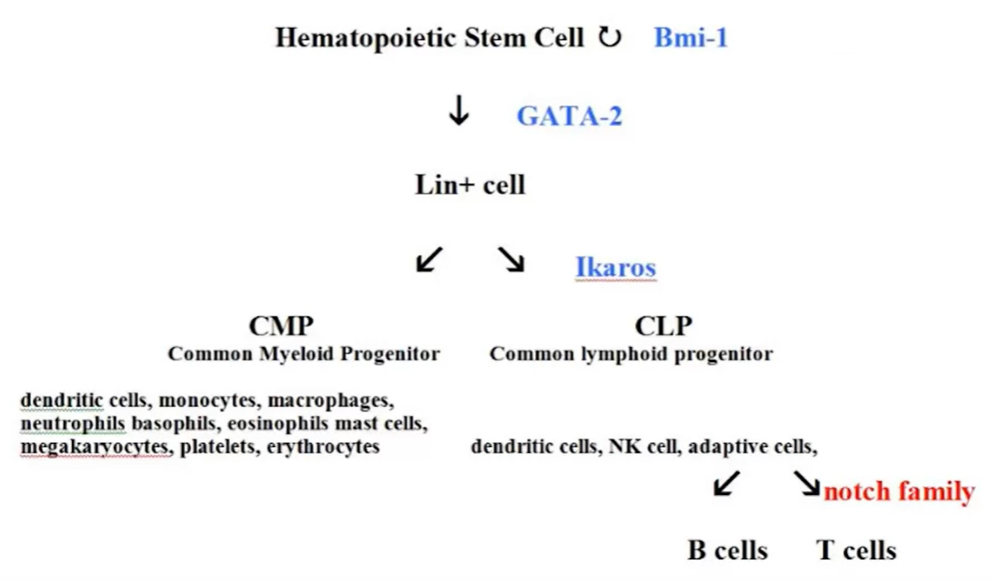
\includegraphics[scale=0.5]{2.2.1.png}
\end{center}
\end{itemize}
2.3\quad \textbf{Myeloid Granulocytes}
\begin{itemize}
\item \concept{Granulocytes} have granules and funky-looking nuclei.
\begin{itemize}
	\item \concept{Neutrophil}:
	\begin{itemize}
		\item Initial response to a threat.
		\item Strongly phagocytic, typically only lives for a day.	
		\item Multi-lobe nucleus.
		\item Granules are both acidic and basic.
		\item Has FC receptors that binds the antibody stems and targets threats.
	\end{itemize}
	\item \concept{Basophil}:
	\begin{itemize}
		\item Complex C-shaped nucleus.
		\item Not phagocytic.
		\item Part of the response to worms and environmental threats.
		\item Granules have C-shaped nucleus.
		\item Has FC receptors that hold E-class antibodies and go looking for antigen.
	\end{itemize}
	\item \concept{Mass cell}:
	\begin{itemize}
		\item Tends to stay at one location.
		\item Has lots of granules with histamine.
		\item Signals running nose, mucus production, and itching if has an allergic response.
		\item Nucleus has no lobes.
		\item Works with basophils to respond to worms and environmental pollutants.
		\item Has FC receptors that hold E-class antibodies and go looking for antigen.
	\end{itemize}
	\item \concept{Eosinophil}:
	\begin{itemize}
		\item Has a bilobed nucleus.
		\item Granules are red as they are staining with eosin red and acidic stain.
		\item Also attacks worms.
		\item Weakly phagocytic, most of the time secretes substances from those red staining granules at the warms.
	\end{itemize}
\end{itemize}
\item \concept{Hygiene hypothesis} states that early childhood exposure to particular microorganisms protects against allergic diseases by contributing to the development of the immune system.
\end{itemize}
2.4\quad \textbf{Myeloid Antigen Presenting Cells}
\begin{itemize}
\item Myeloid antigen presenting cells:
\begin{itemize}
	\item \concept{Monocyte}:
	\begin{itemize}
		\item Makes lot of inclusions and other molecules important in hydrolyzing pathogens, breaking them up, and using them to alert $\mathrm{T_H}$ cells.
		\item Not only phagocitize but also reach out and attempt to transmit information or grab pathogens.
		\item Mobile and has active surface, strongly phagocytic.
	\end{itemize}
	\item \concept{Sentinel Dendritic Cell}:
	\begin{itemize}
		\item First to present an antigen to naive $\mathrm{T_H}$ cells.
		\item Gatekeepers that decide whether or not a $\mathrm{T_H}$ cell will respond to a new antigen.
		\item Not migrating but lying in wait in a tissue to phagocytize antigen, digest it, and then present it to a $\mathrm{T_H}$ cell.
		\item Some belong to the lymphoid lineage.
	\end{itemize}
	\item \concept{Follicular dendritic cell}:
	\begin{itemize}
		\item Incredible number of extensions that can trap \concept{exosomes}, including particles and antigen-antibody complexes.
		\item Instructs B cells by giving them a chance to bind to a particular antigen-antibody complex and thus get some encouragement in their development.
	\end{itemize}
\end{itemize}
\end{itemize}
2.5\quad \textbf{Lymphocytes}
\begin{itemize}
\item B cells:
\begin{itemize}
	\item Developped in the bursa of Fabricius, which is the dorsal wall of the cloaca (common exit) of both the digestive and urogenital system of the bird. 
	\item Has membrane-bound antibody.
	\item Has class II MHC molecules, part of its their way of communicating with $\mathrm{T_H}$ cells.
	\item When stimulated to divide and develop and secrete antibodies, it becomes much larger and its protein synthesis apparatus will be up-regulated. 
\end{itemize}
\item T cells:
\begin{itemize}
	\item Either becomes \concept{cytotoxic} ($\mathrm{T_C}$) cell or \concept{helper} ($\mathrm{T_H}$) cell. $\mathrm{T_C}$ has CD8 and $\mathrm{T_H}$ has CD4. 
	\item $\mathrm{T_H}$ cells are quite diverse, including $\mathrm{T_H}1$, $\mathrm{T_H}2$, $\mathrm{T_{reg}}$, $\mathrm{T_H}17$, etc.
\end{itemize}
\item NK cells:
\begin{itemize}
	\item Many granules and a round nucleus.
	\item Has a trident of Fas ligand (FASL) that up-regulate apoptosis of the cell it sticks into.
	\item If it synapses with a rogue cell or viral-infected or cancerous cell, it has a lot of ammunition in the form of granzymes (serine proteases promoting cytotoxicity of rogue cells) and perforin (glycoprotein responsible for pore formation in cell membranes) that help to break up the cell and send it into asbestosis.
	\item Has MHC1\footnote{\concept{Major Histocompatibility Complex (MHC)} is a large locus on vertebrate DNA containing a set of closely linked polymorphic genes that code for cell surface proteins essential for the adaptive immune system.} regulator that down-regulates to stop from attacking.
	\item Has FC receptor so that if it finds antibodies stuck in the surface of a cell, it will attack the cell.
	\item In a $\mathrm{T_C}$ cell, the MHC receptor will recognize foreign antigen on MHC1 and attack the cell. If a virus down-regulates the production of MHC so that a $\mathrm{T_C}$ cell cannot be alerted to the presence of foreign antigen, NK cells attack it as well. This process is an innate response.
\end{itemize}
\end{itemize}
2.6\quad \textbf{Primary Organs}
\begin{itemize}
\item Three primary lymphoid organs: bursa, bone marrow and thymus.
\begin{itemize}
\item Bone marrow:
\begin{itemize}
	\item Produces most of the immune cells.
	\item Bone marrow has lots of fat that sends out signals that regulate hematopoiesis.
	\item Produces lymphoid cells.
	\item NK cells arise here and B cells rearrange their genes as part of their development.
	\item T cells start out here and migrate into the thymus to rearrange their genes.
	\item Primarily the femur\footnote{Thigh bone.}, humerus\footnote{Bone of the upper extremity.}, arm bones, hip bones, and sternum\footnote{T-shaped vertical bone that forms the anterior portion of the chest wall centrally.} that do the production of most of blood cells.
\end{itemize}
\item Thymus:
\begin{itemize}
	\item Rearrangement site for the T cells.
	\item Has a cortex (outer layer) and medulla (inner layer). 
	\item T cells start from the cortex. T cell progenitors come in in a relatively undifferentiated state. Then,
	\begin{itemize}
	    \item Rearranging genes occur. If no productive rearrangement is derived, the cell dies off.
		\item They undergo a positive selection in the cortex to make sure they can identify antigen on an MHC molecule. If so, they migrate towards the medulla.
		\item They undergo a negative selection in the medulla to get rid of T cells that recognize our own self antigens to prevent auto-immune diseases. 
	\end{itemize}
	Cells pass the three tests leave the circulation and head out to the secondary lymphoid organs to coordinate your immune response, and cells do not pass any of the test will die. Over 95\% of the cells undergo apoptosis as part of this process.
\end{itemize}
\end{itemize} 
\end{itemize}
2.7\quad \textbf{Secondary Organs}
\begin{itemize}
\item The secondary organs of the immune system form an interconnected surveillance system where the immune cells gather and exchange information, including the fluid, vessels and nodes.
\item Circulation involves both the blood vessel (round trip) and the lymph (one-way from the organs out). The plasma from the blood filters into the tissues carrying the proteins, only the lymphoid cells crossover but not the blood cells or myeloid cells.  
\item The lymphatic system picks up fluid throught the body. This drained interstitial fluid from tissues picking up lots of information is gathered up and filtered through the lymph nodes where the antigen is trapped and acted on. Eventually, these vessels grow into larger ones that in turn empty into\footnote{Flows into.} the thoracic duct, left subclavian vein, and then the heart to rejoin the blood circulation.
\item The lymph system also extends into the head, named as the \concept{meningeal system}. It connects with the deep cervical or neck lymph nodes. It lies between the dura mater and the meninges outside the brain and between the meningial arteries and the dural sinuses, which are the veins. The sagittal sinus over the top of the head, transverse sinuses runnning along the side, a lymph vessel is buried in there. It will divide into two transverse branches that contains valves only in the skull, leading out to the cervical lymph nodes. 
\item Fluids come into a lymph node and come out from the efferent vessel. The cortex of a lymph node holds the follicles and the B cells, the power cortex refers to the structure below the cortex, and the medulla sits inside.
\item B cells activated by antigen are to wind up in follicles. The germinal center is where the B cells develop in response to signals from the follicular dendritic cells, $\mathrm{T_H}$ cells, and macrophages will clean up the debris. B cells learn how to bind more tightly to the particular pathgenic antigen here.
\end{itemize}
2.8\quad \textbf{Other Secondary and Tertiary Organs}
\begin{itemize}
\item The lymph nodes, spleen, and gut mucosa are all secondary lymphoid organs. \begin{itemize}
	\item Spleen:
	\begin{itemize}
		\item Lies above the abdomen.
		\item Filters and monitors blood but not lymph.
		\item Has red pulp tissue where the macra fascias recycle old red blood cells.
		\item Has white pulp tissue where T cells participate in immune surveillance.
		\item Has a marginal zone that has B cells in follicles.
	\end{itemize}
	\item \concept{Mucosal Associated Lymphoid Tissue (MALT)} is a collection of tissues including \concept{Bronchial Associated Lymphoid Tissue (BALT)}, \concept{Nasal Associated Lymphoid Tissue (NALT)}, and \concept{Gut Associated Lymphoid Tissue (GALT)}.
	\item The tonsils, appendix, and Peyer's patches (bunch of follicles) in the intestine of some animals also participate in the activation of B cells.
	\item GALT:
	\begin{itemize}
		\item Picks up antigens from the lumen and transports into a developping follicle. Similar in aforementioned other issues.
		\item M cell is sequestering a bunch of immune function cells to facilitate information flow.
	\end{itemize}
\end{itemize}
\item The skin forms a tertiary organ:
\begin{itemize}
	\item Made up of the epidermis, epithelial tissue that sits on a basement membrane, and dermis.
	\item The epidermis derives from embryonic ectoderm, and the dermis derives from embryonic mesoderm. The skin is produced by combining cells from two different tissue layers. It secrets lots of commounds to protect us from pathogenic attack.
	\item Keratinocytes are epithelial cells that upon death retains the keratin and helps to make the skin waterproof. They also express MHC2 and present antigen to T cells. Setenal dendritic cells phagocytizes antigens here as well that can leave the epidermis and go off and look for T cells someplace else.
	\item There is a speical kind of T cells reside in the epidermis and other mucosal tissues that have special receptors. They have built-in quasi-innate recognition for the possible dangerous organisms.
\end{itemize}
\end{itemize}
2.9\quad \textbf{Final Issues}
\begin{itemize}
\item \concept{Apoptosis} is a controlled way of killing off a cell and disposing of the contents.
\item \concept{Necrosis} means a cell swelling, breaking open, spilling its guts, and causing inflammaton.
\end{itemize}
\newpage
\noindent 3.3\quad \textbf{Innate Targeting of Pathogens}
\begin{itemize}
\item People tend to only recognize few protein molecules innately, including 
\begin{itemize}
	\item \concept{Flagellin} that makes up bacterial flagella.
	\item \concept{Profilin} that turns out to be the one that people use to help organize microfilaments.
	\item \concept{$\beta$ 1-3 glucan} that is part of fungi cell-coating.
	\item \concept{Peptidoglycan} that is often found in the cell wall of gram-positive bacteria.
	\item \concept{Lipopolysacchride (LPS)} that is a strong trigger of pattern recognition reception that leads to an inflammatory response.
\end{itemize}
\item Human can also recognize wrong kinds of nucleic acids: ssDNA, dsRNA, or DNA with long methylation patterns.
\item Protective molecules:
\begin{itemize}
	\item Lysozyme can break up peptidoglycan.
	\item Psoriasin found on skin is against E.coli. Too much of it exposed on sunlight can trigger eczema.
	\item Mannose-binding lectins in the plasma.
	\item C-reactive protein recognizes microbes and damaged self cells. It is a sign of general long-term inflammation and is associated with heart attack.
	\item \concept{Nucleotide-binding oligomerization domain (NOD) proteins} in cytoplasm sometimes bind nucleic acid and sometimes bind cell wall compounds.
	\item \concept{Toll-like receptors (TLR)} represents a huge family of molecules. It recognizes parasitic surface proteins using leucine-rich hooks extending into the exterior of the cell and can trigger inflammatory response that will activate NF-kB, a transcription factor that will turn on many genes to fight various infections.
	\begin{itemize}
		\item Plasma membrane TLR recognizes surface characteristics of pathogens, such as cell wall, capsule compounds and flagella.
		\item Endosome TLR recognizes pathogenic nucleic acids after their release during digestion.
	\end{itemize}
	\begin{itemize}
		\item Some is found in the plasma membrane, and the other in endomembranes.
		\item They trigger the recognition of a threat in phagocytic organisms and that is partly what send them off to present antigen to a $\mathrm{T_H}$ cell.
	\end{itemize}
\end{itemize}
\end{itemize}
3.4\quad \textbf{Myeloid Cell Function}
\begin{itemize}
\item After phagocytosis, pathogens in the phagolysosome die when their cell membranes are punctured by \concept{defensin} and their organic molecules are oxidized by HOCl.
\item A compound in the membrane of the phagolysosome takes NADPH and takes the hydrogen off of it to generate $\mathrm{H_2O_2}$. This is an oxidative process, considered to be a form of respiration. It is not generating ATP but some toxic compounds to kill off pathogens. When a neutrophil or a micropahge pahgocytizes a bacterium, a \concept{respiratory burst} takes place, a rapid oxygen uptake as the enzymes are activated. Simultaneously, intake of $\mathrm{K}^+$ takes place to make the vacuole hypertonic. Outside the membrane, we also polymerize actin that acts like a mini-cell wall to keep it from swelling.
\item Several toxic compounds:
\begin{itemize}
	\item Reactive oxygen species:
	\begin{itemize}
		\item Superoxide radicals: $\mathrm{\dot{O}_2}^-$.
		\item Hydrogen peroxide: $\mathrm{H_2O_2}$.
		\item Hypochlorous acid: HOCl.
	\end{itemize}
	\item Reactive nitrogen species:
	\begin{itemize}
		\item Nitric oxide: $\mathrm{NO\cdot}$.
		\item RNS thiols: RNSO.
		\item Peroxynitrous oxide: ONOOH. 
	\end{itemize}
\end{itemize}
\item Though the previous mechanism can kill off most pathogens, some may be able to survive and use macrophages to transport, like tuberculosis and leprosy.
\end{itemize}
3.5\quad \textbf{Quizzes}
\begin{itemize}
\item Neutrophils leave the blood vessels
and enter into infected tissue via a multistep process.
\begin{center}
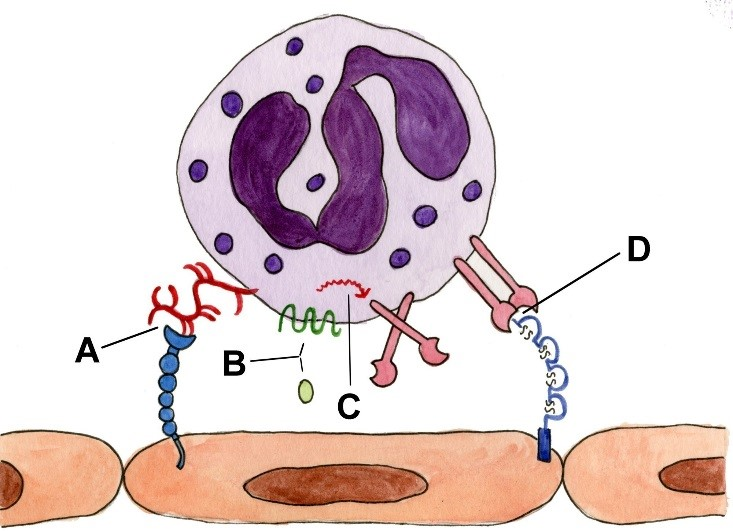
\includegraphics[scale=0.75]{3.5.1.png}
\end{center}
\begin{itemize}
	\item[A:] It indicates the non-covalent linkages between the blue lectin and the red mucin. As these are made and broken the neutrophil sticks and releases from the
endothelium, causing it to roll.
	\item[B:] It indicates the chemokine signal from the endothelium to the
neutrophil, which will lead to internal changes in that cell.
	\item[C:] It indicates the internal cascade pathway kicked off by the chemokine receptor leading to conformational and organizational changes in the neutrophil.
	\item[D:] It indicates the specific conformation of the integrin that allows it to form a tight non-covalent link to the immunoglobulin CAM, leading to arrest, a full stop, not a roll.
\end{itemize}
\item Sleeping sickness and Chagas, malaria, and giardia and leishmaniosis are all caused by eukaryotic trypanosomes whose flagellae are different from that of the prokaryotes.
\end{itemize}
\newpage
\noindent 4.2\quad \textbf{The Immunoglobulin Superfamily}
\begin{itemize}
\item The \textcolor{magenta}{immunoglobulin domain} is referred to a region of the protein where the peptide has folded back up so that hydrophobic parts are inside, hydrophilic parts are outside, and they are stabilized with a disulfide bond. A typical immunoglobulin protein in the subfamily has one or more of these domains, and is typically embedded in the plasma membrane.
\end{itemize}
4.3\quad \textbf{Ig Receptors and Antibodies}
\begin{itemize}
\item If you take blood plasma and put it in electrophoresis apparatus, you get again a series of peaks:
\begin{itemize}
	\item The first peak is \pink{albumins}: about 60000 molecular weight small blood proteins that help carry things around and also keep blood osmotic pressure under control.
	\item The other peaks are called $\alpha_1$, $\alpha_2$, $\beta$ and $\gamma$, respectively.
	\item These proteins are called \pink{globulins} because they are soluble, in contrast to fibrous proteins which are not soluble.
\end{itemize}
\end{itemize}
4.4\quad \textbf{Form and Function}
\begin{itemize}
\item A typical antibody has two Fab fragments, a Fab$_2$ fragment, and a Fc fragment:
\begin{itemize}
\item A Fab fragment is also known as light chain\footnote{A \pink{chain} in immunology is a synonym for peptide.} with molecular weight about 50k.
\item Fab$_2$ fragment and Fc fragment forms a heavy chain with molecular weight about 100k.
\item Fc parts of antigens are very similar, but loop regions at the end of the antibody tends to be variable.
\item A carbohydrate (oligosaccharides) as part of the Fc stage is attached the second chain from the C-terminal and pulls apart the heavy domains in the Fc, whose main significance is in signalling to other parts of the immune system just how to treat whatever this antibody is hooked up against.
\end{itemize}
\item A light chain is a joint of a constant region and a variable region. The whole light chain can either be $\kappa$ or $\lambda$, dictated by two different genes. Human has 4 different choices to put into the $\lambda$. Any cell can either make the $\kappa$ or the $\lambda$, that is, the two light chains in an antibody have to be the same type.
\item There are 5 different types of antibodies, based on the specificity of heavy chains. However, any heavy chain (also pick by that specific cell) can be associated with any light chain, which renders the antibody the capability of binding different antigens.
\end{itemize}
4.5\quad \textbf{Immunoglobulin Classes}
\begin{itemize}
\item There are two major classes of immunoglobulins. Both of them have the variable chain, one constant domain called C1, either a hinged region or another constant domain (C2) that tells the classes apart, and the Fc stem region that has two constant domains, C2 (C3) the bendy ones and C3 (C4) the rigid ones.
\item The hinged region turns out to be a string of prolenes that are stabilized by typically two disulfide bonds.
\item The bottom is the C-terminus of this antibody where attached to the membrane.
\end{itemize}
\newpage
\noindent 4.6\quad \textbf{Specific Ig Types}
\begin{itemize}
\item Antibody classes:

\begin{tabular}{m{0.5cm}<{\centering}m{0.5cm}<{\centering}m{1cm}<{\centering}m{0.8cm}<{\centering}m{0.8cm}<{\centering}m{2cm}<{\centering}m{1.6cm}<{\centering}m{4cm}<{\centering}} \Xhline{1.2pt}
\centering
Ab type \et hinge or rigid \et forms complexes \et J chain \et sub-classes \et timing \et membrane-spanning Ig receptor \et role \\ \hline
M \et rigid \et yes \et yes \et  no \et first class produced in maturing B cells \et yes, naive and memory \et general; activates complement, summons phagocytes, crosses epithelia \\ \hline
D \et hinge \et no \et no \et no \et produced as Ig receptor on mature but naive B cells \et on naive cells, rarely soluble or memory \et aids naive B cell activation \\ \hline
G \et hinge \et no \et no \et 4 \et after class switching in activated B cells \et memory cells only \et specific responses to acute infections \\ \hline
A \et hinge \et yes \et yes \et 2 \et after class switching in activated B cells \et memory cells only \et crosses epithelia, protects boundaries \\ \hline
E \et rigid \et no \et no \et no \et after class switching in activated B cells \et memory cells only \et T$_\mathrm{H}$2 response: defense against worms pollutants \& chronic infections; allergies \\ \Xhline{1.2pt}
\end{tabular}
\\
\item G-class antibodies:
\begin{center}
\begin{tabular}{m{1cm}<{\centering}m{2cm}<{\centering}m{1.5cm}<{\centering}m{1.5cm}<{\centering}m{5cm}<{\centering}} \Xhline{1.2pt}
Class \et hinge length (\# disulfides) \et complement activation \et phagocyte activator \et function \\ \hline
1 \et 2 \et strong \et very strong \et inflammatory: T$_{\mathrm{H}}$1 response to serious threats \\ \hline
2 \et 4 \et weak \et no \et only mildly inflammatory; may cooperate with A and E antibodies during T$_{\mathrm{H}}$2 responses \\ \hline
3 \et 11 \et very strong \et very strong \et highly inflammatory: T$_{\mathrm{H}}$1 response to intracellular pathogens \\ \hline
4 \et 2 \et no \et strong \et intermediate response (possibly mop-up) \\ \Xhline{1.2pt}
\end{tabular}
\end{center}
\item M class antibody is secreted with the J chain (which allows molecules to cross the epithelia) and in an association of typically five of the units put together with disulfide bonds.
\item A class antibody comes with 2 sub-classes. They can be found on the membrane but also secreted in dimers/trimers. They can go to mucus, tears, saliva, breast milk, and one can make up to 15 grams of this a day. It is as a barrier to an assortment of pathogens that prevents one from getting sick. Sometimes bacteria can make protease to attach the hinge region of this antibody to fight it off.
\item E class antibody only occurs in the form of monomer. Its Fc region attaches and even pre-attaches to the FC receptors of basophils, mast cells and eosinophils. 
\end{itemize}
4.7\quad \textbf{Immunoglobulins in Action}
\begin{itemize}
\item \pink{Haptens} are something that is too small to cross-link two receptors in a B cell.
\item Haptens are too small to be immunogenic, so we can manipulate by sticking lots of haptens to enlarged proteins such as bovine serum albumin or BSA.
\end{itemize}
4.8\quad \textbf{Fc Biological Activity}
\begin{itemize}
\item An antibody, instead of summoning basophils, phagocytes, etc., can also activate the \pink{complement} system, part of the immune system that enhances the ability of antibodies and phagocytic cells to clear microbes and damaged cells from an organism, promote inflammation, and attach the pathogen's cell membrane.
\item \pink{Antibody-dependent cellular cytotoxicity (ADCC)} is a mechanism of a cell-mediated immune defense whereby an effector cell of the immune system kills a target cell, whose membrane-surface antigens have been bound by specific antibodies. 
\item J chains of the A and M classes antibodies can trigger \pink{transcytosis}, a type of transcellular transport in which various macromolecules are transported across the interior of a cell, by providing a hook for a membrane embedded transport protein to pick up an antibody complex and transport it from the plasma, across the epithelia, and into gut or breast milk.
\item \pink{Idiotype} is a shared characteristic between a group of immunoglobulin or T-cell receptor (TCR) molecules based upon the antigen binding specificity and therefore structure of their variable region. For example, it can refer to an M class antibody and an A class antibody that have the same N-terminus of the variable chain.
\item \pink{Isotype} can refer to the same class of antibodies that are bound to different antigens (different N-terminus of the variable chain).
\end{itemize}
4.9\quad \textbf{The B Cell Receptor}
\begin{itemize}
\item Immunoglobulin receptors are just Ig antibodies stuck on cell membrane. They can slide aside the cell membrane but not getting out or in. When B cells recognize foreign antigens, they recognize it when two neighboring receptors will bind to that antigen and cross-link. A single receptor cannot begin the signalling process because their cytoplasmic regions are short and don't contain any signalling domains.
\item \pink{CD79A} and \pink{CD79B} (previously known as Ig$\alpha$ and Ig$\beta$) form a hetero-dimer on the plasma membrane that appears next to an Ig molecule, joined by a disulfide bond. Their cytoplasmic region, specifically a region called \pink{immuno-tyrosine activation motifs (ITAMs)}, can pick up a covalent phosphate (put on a tyrosine) and trigger a response.  
\item One can actually make memory cells for all the different classes of antibodies. These memory cells will lie in wait in case that antigen shows up again. Once a class switches away from the naive cells, from then on, in whatever class of antibody one is producing, that is the only class of receptor present in the surface of the cell.
\end{itemize}
4.10\quad \textbf{Monoclonal Antibodies}
\begin{itemize}
\item Typically, a B cell can only live for several weeks. What we can do to make it immortal is via \pink{hybridoma}, that is, to fuse a desired B lineage cell with a B cancer cell:
\begin{itemize}
	\item Put B cells extract from plasma together with \pink{myeloma} cell (B cancer cell) that makes no antibody in polyethylene glycol (to disrupt membranes), and they tend to fuse together.
	\item Put them into an \pink{hypoxanthine aminopterin thymidine (HDT)} medium. As rapidly dividing cells, these cells need to make DNA. There are several pathways for these cells to do this: a de novo pathway to make everything from scratch, or a salvage pathway to pick up materials to salvage them (here supplied by hypoxanthine and thymidine). Here, aminopterin can block the de novo pathway so that only the hybridoma can be retained, as myeloma cells cannot reproduce via the salvage pathway.
	\item Engineer the antibody-producing cells to make a human, not a mouse antibody.
\end{itemize}
\end{itemize}
4.11\quad \textbf{Quizzes}
\begin{itemize}
\item \pink{Adjuvant} is a substance that increases or modulates the immune response to a vaccine. The most common category of adjuvants in US vaccines is aluminum salts, which activate cytoplasmic NOD receptors to improve the effectiveness of antibody production. Bacterial cell wall peptides have been used in the past, but these can produce an excess inflammatory response.
\item \pink{Mercaptoethanol} can reduce the disulfide bonds; pepsin is an endopeptidase that breaks down proteins into smaller peptides.
\end{itemize}
\newpage
\noindent 5.1\quad \textbf{Uniqueness of the System}
\begin{itemize}
\item \pink{Chromatin diminution} is defined as chromosomal fragmentation followed by the elimination of part of the chromosome during mitosis in somatic cells.
\item Ig gene rearrangement can make a vast number of antibodies (at order $10^8\sim 10^{11}$), which does the process involve enzymes reading specific signals in 6 or fewer genes.
\end{itemize}
5.3\quad \textbf{Gene to RNA to Protein}
\begin{itemize}
\item A diploid human cell has 2 heavy, 2 $\lambda$-light, and 2 $\kappa$-light genes.
\end{itemize}
5.4\quad \textbf{Light Chain Gene Expression}
\begin{itemize}
\item Human $\lambda$-light chain gene lies on chromosome 22, and $\kappa$-light gene lies on chromosome 2.
\item A $\lambda$-light chain gene is composed of many V fragments (number differs across individuals but around 30), each preceded by an L region, and then 5 C regions, each preceded by a J region. To make different light chains, any V fragment can be stuck before a J fragment so that only the preceding promoter (L region) will be activated and thus start transcription to a "stop" signal that is somewhere in between the C region and next J region.
\item A $\kappa$-light chain gene is composed of many V fragments (number differs across individuals but around 40), each preceded by an L region, and then a constant C region, preceded by 5 J regions. The way to produce a $\kappa$-light chain is similar to the previous one, but since the $\kappa$-light gene has only 1 constant region, any J fragments in between the attached J region and the constant region will be removed from the mature message during splicing process.
\end{itemize}
5.5\quad \textbf{Heavy Chain Gene Expression}
\begin{itemize}
\item Human heavy chain gene lies on chromosome 14.
\item A heavy chain gene is composed of many V fragments (number differs across individuals but around 40), each preceded by an L region, many D fragments (number differs across individuals but around 20), 5 J regions and 9 C fragments. 
\begin{itemize}
	\item Of the 9 C fragments, each is followed by a membrane spanning region, and except for the first C$_\mu$ region, each of the rest is followed by a transcriptional stop signal.
	\item To make different heavy chains, any V fragment can be stuck before a D fragment, followed by any J, so that only the preceding promoter (L region) will be activated and thus start transcription to any transcriptional stop signal after the 8 C regions. Note that though the C$_\mu$ region is always included in the primary transcript, only one C region can be present in the final message passed to translation.
	\item The final C region dictates which class (M, D, A, E, or G) this antibody belongs to.
	\item They will form the early Ig receptors on naive but mature B cells.
\end{itemize}
\end{itemize}
5.6\quad \textbf{Rearrangement in Developmental Context}
\begin{itemize}
\item The development of the mature B cell and then plasma cell:
\begin{itemize}
	\item It begins with the lymphoid progenitor in the bone marrow. The lymphoid progenitor is derived by stimulating hematopoietic stem cells.
	\item Signalling molecules (Ig$\alpha$ and Ig$\beta$) are synthesized and put into the membrane. At this stage, this is named as a \pink{pro-B cell}.
	\item The cell is sent to the B pathway by hitting with BSAP, which will trigger the rearrangement of the heavy chain gene (remember, this will be an IgM). If both copies of genes do not work, this cell will undergo apoptosis. At the same time, the production of a fake (surrogate) light chain is up-regulated, combined with the heavy chain, and stuck to the membrane for signalling that this cell is ready to go to the next stage. At this stage, this is named as a \pink{pre-B cell}. Also, one can find CD25 ($\alpha$ chain of IL-2 receptor) on the surface of this cell.
	\item Then, nucleus will rearrange. It will try to make the $\kappa$-light chain twice before the $\lambda$-light chain, again twice. If all four attempts fail, the cell goes to apoptosis. Provided succeeding, the fake Ig receptor will recycle during normal membrane turnover so that the real light chain is attached. After this new molecule is stuck to the membrane, the cell becomes an immature B cell.
	\item Before the cell becomes a mature B cell, it has to make sure that it's not recognizing any self-antigen. If so, Ig$\alpha$ and Ig$\beta$ will signal for apoptosis. If the cell passes this test, it'll signal for activating the cell instead of commit suicide.
	\item Now, IgD can be synthesized. The cell becomes a mature but naive\footnote{It is considered naive because it is still stuck in the bone marrow.} B cell.
	\item The cell leaves the bone marrow and enter the circulation.
	\begin{center}
	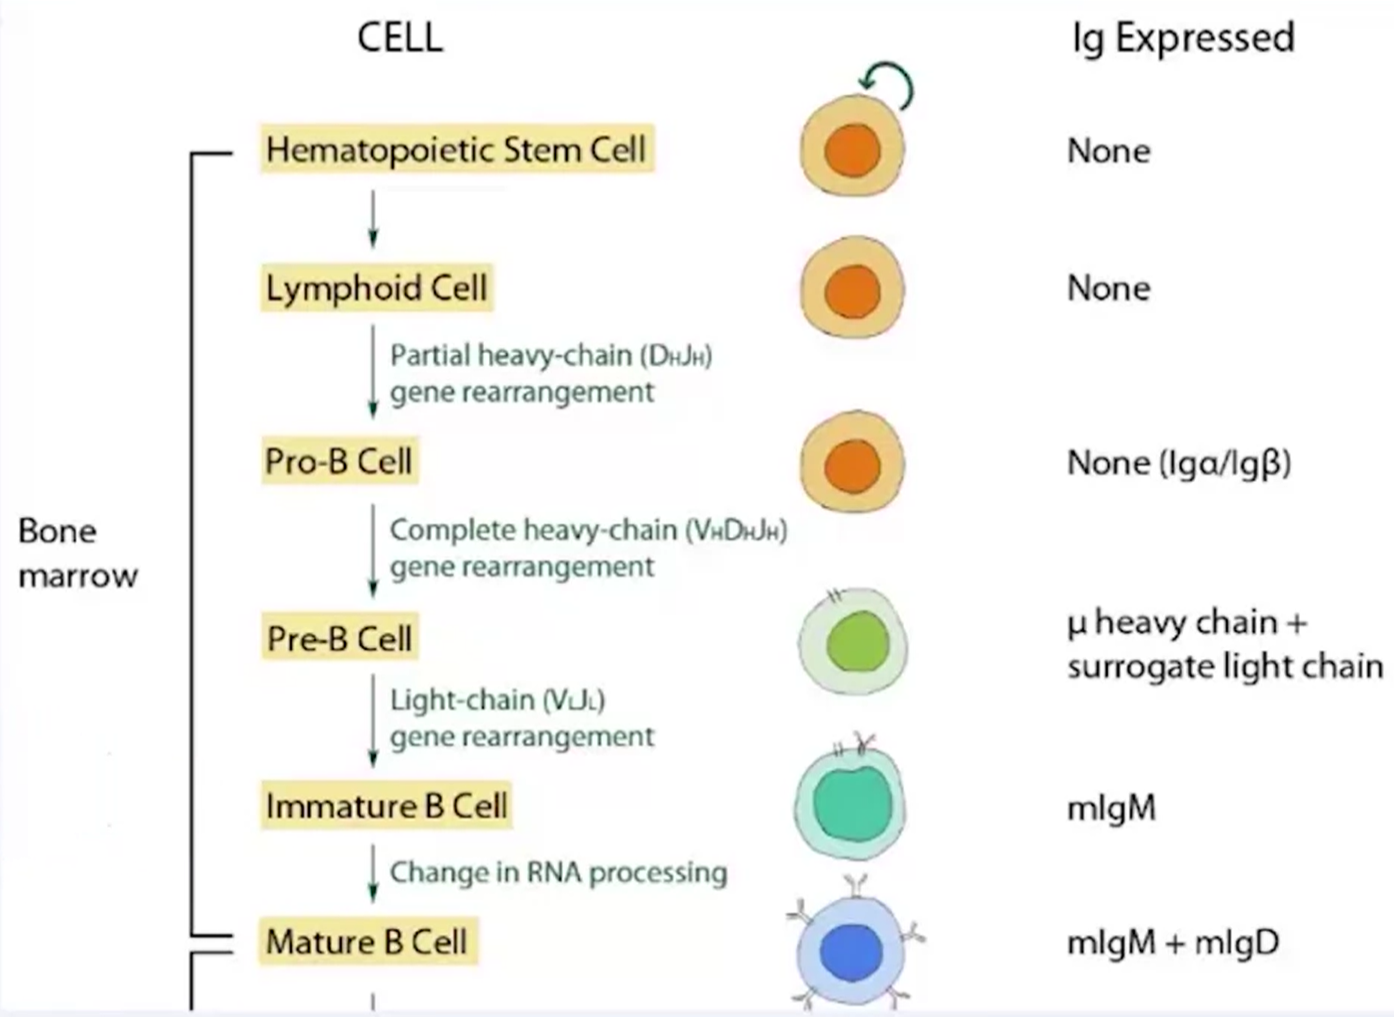
\includegraphics[scale=0.35]{5.6.1.png}
	\end{center}
\end{itemize}
\item \pink{Somatic hypermutation} is a process in which point mutations accumulate in the antibody V regions of both the heavy and light chains, at rates that are about 
$10^6$-fold higher than the background mutation rates observed in other genes.
\end{itemize}
5.7\quad \textbf{Recombination Signal Sequence Structure}
\begin{itemize}
\item Recombination Signal Sequence:
\begin{itemize}
	\item They are on different side of different regions:
	\begin{itemize}
		\item V regions have downstream signal sequences. They are not identical but similar.
		\item D regions have both up and down signal sequences.
		\item J regions have upstream signal sequences.
		\item C regions do not have any signal sequence.
	\end{itemize}
	\item They can be even longer for the constant/variable fragments. For example, the D region is only 9bps long, but the flanking sequences\footnote{In molecular biology, flanking sequence refers to the nucleotide sequences adjacent to a specific DNA sequence of interest.} are longer than that.
	\item A signal sequence is composed of a heptamer (a palindrome), a 12bps (for Vs)/23bps (for Js)\footnote{This actually is in $\kappa$-light chain genes. In $\lambda$-light chain genes, this is flipped.} sequence, and an AT-rich nanomer\footnote{From 5' to 3' for Vs, and from 3' to 5' for Js.}. Only different middle sequences can be put together to prevent two Vs or Js are put together. In a heavy chain, Vs and Js are surrounded by 23bps sequence, will both sides of the Ds are surrounded by 12bps sequence.
\end{itemize}
\item These signal sequences can help the DNA attach to, and be moved around, and chemically rearranged by a enzyme complex called \pink{V(D)J recombinase}.
\end{itemize}
5.8\quad \textbf{Mechanism Details}
\begin{itemize}
\item To bring about gene rearrangement of the heavy and light chains, we first randomly cut the heptamer succeeding a V region and the corresponding heptamer preceding a J region on the other strand of the DNA molecule (needless to say, it does not have to be joining these two). The free end of the palindromic regions will attack the other strands to form an ssDNA loop, and nucleotides in between the loops will then be removed. The ssDNA loops will then be held by the enzyme complex, which in turn is to clip the loops in no necessarily corresponding places. After ligating the open ends of the same strands, one strand can have longer DNA than the other, so to form a double helix, the missing bit of DNA will have some nucleotides (according to base pairing) attached to complete the ligation process, that is, \pink{P-nucleotide addition}.
\item Specifically in the heavy chain gene, the VD and DT joints can be opened up and added in a number of nucleotides at random, known as \pink{N-nucleotide addition}.
\end{itemize}
5.9\quad \textbf{Commitment to a Definite CDR}
\begin{itemize}
\item \pink{Allelic exclusion} is a process by which only one allele of a gene is expressed while the other allele is silenced. If the rearrangement process succeeds in making some functional products, the other strand will be silenced.
\item One of the consequences of the enormous amount of cell division, rearrangement, DNA changes is that mutations happen and leukemias, lymphomas, and other diseases of blood cells may occur.
\end{itemize}
5.10\quad \textbf{Generation of Antibody Diversity}
\begin{itemize}
\item \pink{Complementarity-Determining Regions (CDRs)} are part of the variable chains in Igs. The variable chain folds to form 3 loops, which will be the main points of pathogen detection (and most variable). The first two loops are within the V regions of the light chain gene, whereas the third is mainly at the V-J junction, including the P-nucleotide addition sequences. These loops are where that is most likely to undergo somatic hypermutation. For the heavy chain, it is exactly the same procedure except that the third loop for that CDR is not the V-J junction but D segments.
\end{itemize}
5.11\quad \textbf{Class Switching}
\begin{itemize}
\item In heavy chain gene rearrangement, only the most upstream C segments can be used. Therefore, to express other classes of antibodies, the previous C segments have to be removed first, which means class switching is unidirectional - it cannot reverse to the previous classes. Since each C segments have a stop signal right after it (except C$_\mu$), downstream fragments will not be expressed.
\item The motive to class switch comes from T$_{\mathrm{H}}$ cells. They're going to give cytokines to the B cells, as if saying a not all purpose M class stem is requested, and ultimately interact with enzymes to cleave the undesirable C segments on the heavy chain gene.
\end{itemize} 
\newpage
6.3\quad Activation: Thymus Independent
\begin{itemize}
\item To activate a B cell, one may not have a T$_\mathrm{H}$ cell involved (thus named \pink{thymus-independent reactions}):
\begin{itemize}
	\item Thymus-independent antigens T-1 is the lipopolysaccharide found in the surfaces of gram-negative cells. It also needs to bind a TLR to activate the cell.
	\item Thymus-independent antigens T-2 is the flagellin, capsule polysaccharides around the outside of bacteria, and other large repeating molecules. Since these substances are large, they tend to cross-activate about 10 Igs together. Pro-inflammatory cytokines, IL-2, IL-3, IFN-$\gamma$, with the intervention from either macrophages and sentinel dendritic cells, can also activate a B cell, though they may not be considered as T-2.
\end{itemize}
\item Signal 1 is used by both thymus-independent and thymus-dependent B cells. When an antigen crosslinks the Ig receptors, \pink{src-like kinases} will be recruited to add phosphates to the ITAMs extending into the cytoplasm. Once done, three different kinds of responses can be triggered by \pink{syk-kinases}:
\begin{itemize}
	\item One of the membrane phospholipids will be taken and hydrolyzed into diacylglyceride (DAG) and phosphoinositol (PIP). These compounds trigger:
	\begin{itemize}
		\item Calcium is released in the ER that activates calmodulin, which in turn activates a number of other pathways. One important one is the removal of a phosphate from NFAT which activates it and then NFAT becomes an activate transcription factor, goes into the nucleus, and turns on the genes necessary for the cell to divide and then changes developmental pathway and produce antibodies.
		\item Inhibitor kappa B, from an inactive NF kappa B molecule, is removed. This molecule will also serve as a transcription factor, goes into the nucleus, and up-regulates inflammatory genes for the cell to develop into an active B cell.
	\end{itemize}
	\item A phosphorylation pathway named \pink{RAS-RAF-MEK-ERK pathway} is triggered. The substances are in this turn phosphorylated, and finally ERK activates multiple transaction factors that will then bind to the DNA and promote B cell division and differentiation.
	\item PIP has two phosphates, and when a third phosphate is added, it attracts a bunch of compounds to down-regulate apoptosis.
\end{itemize}
\item On the cell surface of these B cells, there are F$_\mathrm{c}$ receptors that bind to antigen-antibody complexes, which will then in turn down-regulate antibody production.
\end{itemize}
6.4\quad Primary and Secondary Responses: T cells
\begin{itemize}
\item T$_\mathrm{H}$ cells promote the development of B cells stimulating them to divide, possibly improving their antibody binding through affinity maturation; they also assist in class-switching and B cell differentiation (into memory B cells) upon antigen clearance.
\item Upon Ig receptors binding to an antigen, it will internalize the complex via a vesicle, transport into the cytoplasm, fuse with another vesicle that contains MHC-II molecules, digest the antigen, send it back out and present to T$_\mathrm{H}$ cells. This complex will be bound to CD4 and cause the T cell to produce CD154 (or CD40 ligand, abbreviated as CD40L) to bind CD40 receptors on the surface of B cells, followed by triggering the ITAM (and downstreaming) pathways (known as signal 2).
\end{itemize}
6.5\quad Anatomical and Histological Context
\begin{itemize}
\item A follicular dendritic cell has lots of \pink{iccosomes} (antigen-antibody complexes) attached to its cell surface, which will then interact with B cells to trigger immune response.
\end{itemize}
6.6\quad Affinity Maturation
\begin{itemize}
\item The peripheral region of a secondary follicle inside a lymph node is where most B cell undergoes rearrangements to produce different CDR regions (to recognize antigens). Now, mature B cells will move into the center of the follicle and bind the exosomes (iccosomes) on the surface of follicular dendritic cells, where only the B cell receptors with higher affinity can be retained. This is how different CDR regions get selected to produce efficient antibodies.
\item Sentinel dendritic cells signal to T$_\mathrm{H}$ cells using antigen on MHC-II, as well as cytokines that report in on the source of the pathogen. If infected, they could signal to T$_\mathrm{c}$ cells with MHC-I, but that’s much less likely to happen.
\end{itemize}
6.7\quad Final Decisions
\begin{itemize}
\item If a developing B cell decides to become a memory cell, it will up-regulate the production of a splicing enzyme that adds the membrane-spanning exons.
\end{itemize}
6.8\quad Regulation
\begin{itemize}
\item BSAP is a transcription factor expressed only by cells that are currently developing as B cells. BSAP is what induces a lymphoid cell to transform into a B lineage cell. If it becomes a B memory cell, BSAP can still be made. However, if it becomes a B plasma cell, production of BSAP will be ceased.
\end{itemize}
6.9\quad Quizzes
\begin{itemize}
\item Memory cells tend to arise at the end of an infection. Thus, rising levels of antigen and inflammatory cytokines would promote the development of more effector cells. Fats cells operate on B cells during development.
\item After selection of effectiveness, T$_\mathrm{H}$ cell may direct the B cell to leave lymph node and head to the site of an infection and secrete antibodies there, which will cause the B cell to make more rough ER so that it can produce quantities of secreted proteins instead of just several hundred receptors. It need not class switch to do this.
\end{itemize}
\end{document}
